% ------------------------------------------------------------------------------

\begin{frame}[fragile]{Формулы и выкладки}

\begin{itemize}[<+->]
    \item ``Меньше или равно'' и ``больше или равно''
    \item Косые чаще выглядят лучше
    \item Заменим по умолчанию
\end{itemize}

\begin{onlyenv}<1>
    \begin{align*}
        x \leq y \quad y \geq z
    \end{align*}

    \begin{block}{Код}
        \begin{lstlisting}
    \begin{align*}
        x \leq y \quad y \geq z
    \end{align*}
        \end{lstlisting}
    \end{block}
\end{onlyenv}

\begin{onlyenv}<2>
    \begin{align*}
        x \leqslant y \quad y \geqslant z
    \end{align*}
    
    \begin{block}{Код}
        \begin{lstlisting}
    \begin{align*}
        x \leqslant y \quad y \geqslant z
    \end{align*}
        \end{lstlisting}
    \end{block}
\end{onlyenv}

\begin{onlyenv}<3>
    {
        \renewcommand{\leq}{\leqslant}
        \renewcommand{\geq}{\geqslant}
        
        \begin{align*}
            x \leq y \quad y \geq z
        \end{align*}
    }
    
    \begin{block}{Код}
        \begin{lstlisting}
    \renewcommand{\leq}{\leqsant}
    \renewcommand{\geq}{\geqslant}
    
    \begin{align*}
        x \leq y \quad y \geq z
    \end{align*}
        \end{lstlisting}
    \end{block}
\end{onlyenv}

\end{frame}

% ------------------------------------------------------------------------------

\begin{frame}[fragile]{Формулы и выкладки}

\begin{itemize}[<+->]
    \item Пределы
    \item Верхние и нижние пределы
\end{itemize}

\begin{onlyenv}<1>
    \begin{align*}
        \lim_{n \to \infty} \frac{1}{n}
    \end{align*}
    
    \begin{block}{Код}
        \begin{lstlisting}
    \begin{align*}
        \lim_{n \to \infty} \frac{1}{n}
    \end{align*}
        \end{lstlisting}
    \end{block}
\end{onlyenv}

\begin{onlyenv}<2>
    \begin{align*}
        \varlimsup_{n \to \infty} \frac{1}{n^2} \quad
        \varliminf_{n \to \infty} \frac{-\pi}{\log n}
    \end{align*}
    
    \begin{block}{Код}
        \begin{lstlisting}
    \begin{align*}
        \varlimsup_{n \to \infty} \frac{1}{n^2} \quad
        \varliminf_{n \to \infty} \frac{-\pi}{\log n}
    \end{align*}
        \end{lstlisting}
    \end{block}
\end{onlyenv}

\end{frame}

% ------------------------------------------------------------------------------

\begin{frame}[fragile]{Формулы и выкладки}

\begin{itemize}
    \item Суммы
    \begin{align*}
        \sum_{k = 1}^{n^2} \frac{\log k}{k^2}
    \end{align*}
\end{itemize}

\begin{block}{Код}
    \begin{lstlisting}
    \begin{align*}
        \sum_{k = 1}^{n^2} \frac{\log k}{k^2}
    \end{align*}
    \end{lstlisting}
\end{block}

\end{frame}

% ------------------------------------------------------------------------------

\begin{frame}[fragile]{Формулы и выкладки}

\begin{itemize}[<+->]
    \item Для длинных выражений не забудьте про \lstinline!\left(! и \lstinline!\right)!
    \item Или же \lstinline!\left[! и \lstinline!\right]!
\end{itemize}

\begin{onlyenv}<1>
    \begin{align*}
        \sum_{k = 1}^{n^2} \left( \frac{\log k}{k^2} + \frac{e^k}{k!} \right)
    \end{align*}
    
    \begin{block}{Код}
        \begin{lstlisting}
    \begin{align*}
        \sum_{k = 1}^{n^2} \left( 
            \frac{\log k}{k^2} + \frac{e^k}{k!} 
        \right)
    \end{align*}
        \end{lstlisting}
    \end{block}
\end{onlyenv}

\begin{onlyenv}<2>
    \begin{align*}
        \sum_{k = 1}^{n^2} \left[ \frac{\log k}{k^2} + \frac{e^k}{k!} \right]
    \end{align*}
    
    \begin{block}{Код}
        \begin{lstlisting}
    \begin{align*}
        \sum_{k = 1}^{n^2} \left[
            \frac{\log k}{k^2} + \frac{e^k}{k!} 
        \right]
    \end{align*}
        \end{lstlisting}
    \end{block}
\end{onlyenv}

\end{frame}

% ------------------------------------------------------------------------------

\begin{frame}[fragile]{Формулы и выкладки}

\begin{itemize}[<+->]
    \item Интегралы
    \item Пределы снизу и сверху
    \item Двойные интегралы по множеству
    \item Интеграл по контуру
\end{itemize}

\begin{onlyenv}<1>
    \begin{align*}
        I(\alpha) = \int_{0}^{+\infty} f(x, \alpha) dx
    \end{align*}

    \begin{block}{Код}
        \begin{lstlisting}
    \begin{align*}
        I(\alpha) = \int_{0}^{+\infty} f(x, \alpha) dx
    \end{align*}
        \end{lstlisting}
    \end{block}
\end{onlyenv}

\begin{onlyenv}<2>
    \begin{align*}
        I(\alpha) = \int\limits_{0}^{+\infty} f(x, \alpha) dx
    \end{align*}

    \begin{block}{Код}
        \begin{lstlisting}
    \begin{align*}
        I(\alpha) = \int\limits_{0}^{+\infty} f(x, \alpha) dx
    \end{align*}
        \end{lstlisting}
    \end{block}
\end{onlyenv}

\begin{onlyenv}<3>
    \begin{align*}
        \iint\limits_{S} y \, dz \, dx
    \end{align*}

    \begin{block}{Код}
        \begin{lstlisting}
    \begin{align*}
        \iint\limits_{S} y \, dz \, dx
    \end{align*}
        \end{lstlisting}
    \end{block}
\end{onlyenv}

\begin{onlyenv}<4>
    \begin{align*}
        \oint\limits_{ABCDA} \frac{dx + dy}{|x| + |y|}
    \end{align*}

    \begin{block}{Код}
        \begin{lstlisting}
    \begin{align*}
        \oint\limits_{ABCDA} \frac{dx + dy}{|x| + |y|}
    \end{align*}
        \end{lstlisting}
    \end{block}
\end{onlyenv}

\end{frame}

% ------------------------------------------------------------------------------

\begin{frame}[fragile]{Формулы и выкладки}

\begin{itemize}[<+->]
    \item Матрицы, p -- круглые скобки (parenthesis)
    \item b -- квадратные скобки (brackets)
\end{itemize}

\vspace{-0.7cm}

\begin{onlyenv}<1>
    \begin{align*}
        \begin{pmatrix}
            a_{11} & a_{12} & \dots  & a_{1m} \\
            a_{21} & a_{22} & \dots  & a_{2m} \\
            \vdots & \vdots & \ddots & \vdots \\
            a_{n1} & a_{n2} & \dots  & a_{nm}
        \end{pmatrix}
    \end{align*}
    
    \vspace{-0.3cm}
    
    \begin{block}{Код}
        \begin{lstlisting}
    \begin{pmatrix}
        a_{11} & a_{12} & \dots  & a_{1m} \\
        a_{21} & a_{22} & \dots  & a_{2m} \\
        \vdots & \vdots & \ddots & \vdots \\
        a_{n1} & a_{n2} & \dots  & a_{nm}
    \end{pmatrix}
        \end{lstlisting}
    \end{block}
\end{onlyenv}

\begin{onlyenv}<2>
    \begin{align*}
        \begin{bmatrix}
            a_{11} & a_{12} & \dots  & a_{1m} \\
            a_{21} & a_{22} & \dots  & a_{2m} \\
            \vdots & \vdots & \ddots & \vdots \\
            a_{n1} & a_{n2} & \dots  & a_{nm}
        \end{bmatrix}
    \end{align*}
    
    \vspace{-0.3cm}
    
    \begin{block}{Код}
        \begin{lstlisting}
    \begin{bmatrix}
        a_{11} & a_{12} & \dots  & a_{1m} \\
        a_{21} & a_{22} & \dots  & a_{2m} \\
        \vdots & \vdots & \ddots & \vdots \\
        a_{n1} & a_{n2} & \dots  & a_{nm}
    \end{bmatrix}
        \end{lstlisting}
    \end{block}
\end{onlyenv}

\end{frame}

% ------------------------------------------------------------------------------

\begin{frame}[fragile]{Формулы и выкладки}

Live coding: верстаем предел интеграла

\begin{figure}
    \centering
    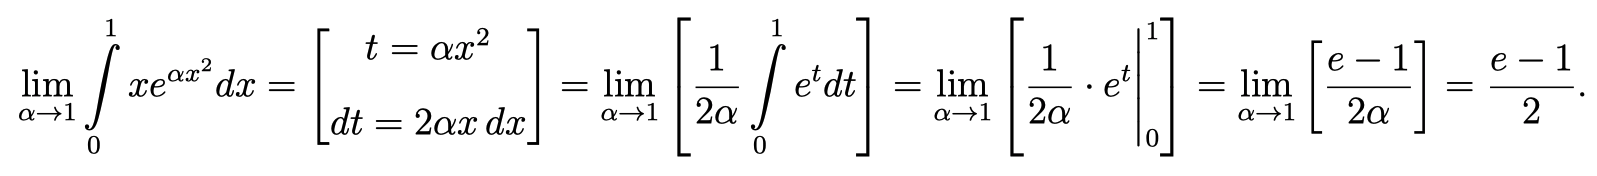
\includegraphics[width=\textwidth]{images/limit-int.png}
\end{figure}

\end{frame}

% ------------------------------------------------------------------------------

\begin{frame}[fragile]{Формулы и выкладки}

\begin{itemize}[<+->]
    \item Множества
    \item Известные множества
    \item Шорткаты
\end{itemize}

\begin{onlyenv}<1>
    \begin{align*}
        B_k = \{ w \mid \eta(w) = \eta_k \}
    \end{align*}
    
    \begin{block}{Код}
        \begin{lstlisting}
    \begin{align*}
        B_k = \{ w \mid \eta(w) = \eta_k \}
    \end{align*}
        \end{lstlisting}
    \end{block}
\end{onlyenv}

\begin{onlyenv}<2>
    \begin{align*}
        \mathbb{N}, \mathbb{Z}, \mathbb{Q}, \mathbb{R}
    \end{align*}
    
    \begin{block}{Код}
        \begin{lstlisting}
    \begin{align*}
        \mathbb{N}, \mathbb{Z}, \mathbb{Q}, \mathbb{R}
    \end{align*}
        \end{lstlisting}
    \end{block}
\end{onlyenv}

\begin{onlyenv}<3>
    \vspace{-0.7cm}
    {
        \newcommand{\N}{\mathbb{N}}
        \newcommand{\Z}{\mathbb{Z}}
        \newcommand{\Q}{\mathbb{Q}}
        \newcommand{\R}{\mathbb{R}}
        \begin{align*}
            \N, \Z, \Q, \R
        \end{align*}
    }
    
    \begin{block}{Код}
        \begin{lstlisting}
    \newcommand{\N}{\mathbb{N}}
    \newcommand{\Z}{\mathbb{Z}}
    \newcommand{\Q}{\mathbb{Q}}
    \newcommand{\R}{\mathbb{R}}
    
    \begin{align*}
        \N, \Z, \Q, \R
    \end{align*}
        \end{lstlisting}
    \end{block}
\end{onlyenv}

\end{frame}
